\section{Motivación del proyecto}
\subsection{Apartado Uno}
\begin{large}
Texto del apartado uno
As shown in \cite{smith2023}, the results are promising.

\begin{itemize}
   \item Item 1
   \item Item 2
   \item Item 3
   \item Item 4
\end{itemize}
\end{large}

\section{Planteamineto}
El TFG consistirá en el despliegue de una infraestructura tecnológica para la captura y el procesamiento de datos públicos, 
junto con el diseño, desarrollo y validación de un modelo predictivo que permita extraer información valiosa a partir de dichos datos.
 Este enfoque integrará tanto aspectos técnicos relacionados con la gestión y el análisis de datos como la aplicación de técnicas predictivas
  basadas en modelos de aprendizaje automático, con el fin de optimizar y automatizar la toma de decisiones en un contexto específico.
\begin{large}
\begin{itemize}
   \item Item 1
   \item Item 2
   \item Item 3
\end{itemize}
\end{large}

\section{Antecedentes y estado del arte}

\begin{large}
Bla, bla, bla.
\end{large}

\section{Objetivos}

\begin{large}
Bla, bla, bla.
\end{large}

\newpage

\begin{figure}[htb]
   \centering
   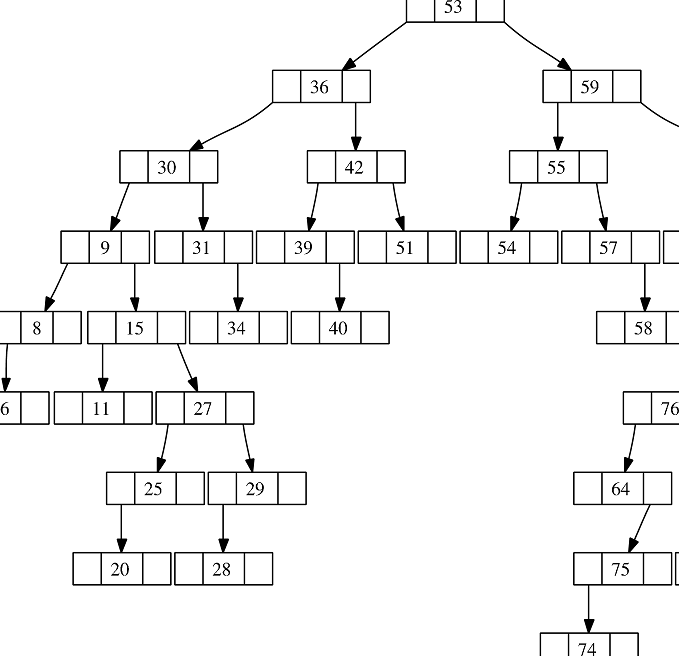
\includegraphics[width=0.8\linewidth]{images/figura_1}
   \caption{Ejemplo de figura}
   \label{chapter:intro}
\end{figure}